\section{Marco teórico}

En esta sección se desarrollarán los principios teóricos que permiten el funcionamiento de las lanzaderas electromagnéticas. Para entender estos principios, es esencial comprender los fundamentos del electromagnetismo, el concepto de bobina y su relación con la generación de campos magnéticos.

El electromagnetismo es una rama fundamental de la física que estudia las interacciones entre los campos eléctricos y magnéticos. Su desarrollo ha sido crucial para el avance de la tecnología, desde la generación y transmisión de electricidad hasta las comunicaciones inalámbricas. Aunque la raza humana conoce los fenómenos eléctricos y magnéticos desde la historia antigua, estos no fueron estudiados hasta el siglo XVII, y se consideraban fenómenos independientes hasta que Hans Christian Ørsted descubrió en 1820 que una corriente eléctrica puede generar un campo magnético. Mientras el físico danés preparaba los equipos para dar una conferencia en la Universidad de Copenhague, observó que la aguja de una brújula cercana se desviaba cuando la corriente fluía a través de un alambre conductor. Este accidental descubrimiento le llevó a publicar el artículo CIRCA EFFECTUM CONFLICTUS ELECTRICI IN ACUM MAGNETICAM, en el que se describieron los fenómenos electromagnéticos por primera vez, aunque de manera cualitativa. En la siguiente década, Ampère y Faraday describirían matemáticamente el descubrimiento de Ørsted, dando lugar al electromagnetismo como lo conocemos hoy en día. \citep{oersted2024}

El trabajo de James Clerk Maxwell en la década de 1860 unificó estos descubrimientos en un marco teórico coherente. Maxwell formuló un conjunto de ecuaciones que describen cómo los campos eléctricos y magnéticos interactúan y se propagan. Estas ecuaciones, conocidas como las ecuaciones de Maxwell, son la base del electromagnetismo clásico.

\begin{figure}[H] % Use H specifier to place exactly here
    \centering
    \[
    \vec{\nabla}\cdot \vec{E}= \frac{\rho}{\epsilon_0}~~~~~~\vec{\nabla}\cdot \vec{B}= 0
    \]
    \[
    \vec{\nabla}\times\vec{E}=-\frac{\partial\vec{B}}{\partial t}~~~~~~\vec{\nabla}\times \vec{B}=\mu_0\vec{J}+\mu_0\epsilon_0\frac{\partial \vec{E}}{\partial t}
    \]
    \caption{Ecuaciones de Maxwell.\citep{purcell2013electricidad}}
    \label{fig:maxwell_equations}
\end{figure}

\begin{figure}[H]
    \centering %\raggedleft \raggedright
    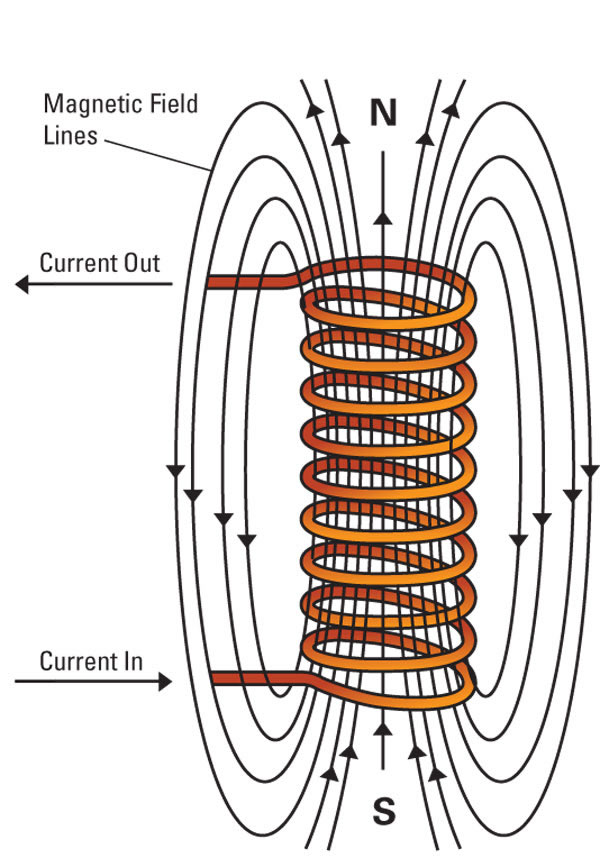
\includegraphics[width=8cm]{FigurasMemoria/fig3electromagnet.jpg}
    \caption{Campo magnético en una bobina. www.lanl.gov}
    \label{fig:2} %Para referenciar -> \ref{fig:figNum}
\end{figure}

Como se ha mencionado en la introducción, el funcionamiento de una lanzadera electromagnética se basa en la capacidad de las bobinas de generar un flujo magnético cuando se les aplica una corriente, como se puede ver en la. Esto es debido a la ley de Àmpere, que enuncia lo siguiente:

\begin{quote}
    Según la ley de Ampère, la integral de línea del campo magnético \(\mathbf{B}\) alrededor de un lazo cerrado es igual a \(\mu_0\) multiplicado por la corriente total \(I_{enc}\) que pasa a través de cualquier superficie delimitada por el lazo. Matemáticamente, esto se expresa como:
    \[
    \oint_{\partial S} \mathbf{B} \cdot d\mathbf{l} = \mu_0 I_{enc}
    \]
    donde \(\mu_0\) es la permeabilidad del vacío.
\end{quote}

La manera más básica de representar una lanzadera es un simple circuito con una fuente de alimentación, un interruptor controlado por un circuito electrónico y una bobina, que es la encargada de generar el campo.